\chapter{Resultados} \label{chap:Resultados}

%Como se observa en la propuesta en el Capítulo \ref{chap:Propuesta}, el reconocimiento de rostros en vídeo vigilancia cuenta con varias partes que intervienen en este proceso. En este capítulo dichas partes son puestas a evaluación y se presentan propuestas de mejora y se explica sus resultados experimentales.
En este capítulo se muestran los los resultados de investigación de la presente tesis, el presente capítulo se divide en dos partes. La primera parte son las base de datos con las que se ha trabajado, donde las tres primeras fueron utilizadas para las pruebas iniciales de la investigación, para realizar comparativas entre métodos de reconocimiento de rostro y el análisis paramétrico que se realizó después, mientras que la ultima base de datos fue hecha para las pruebas finales de la propuesta, finalizando la primera parte se explica el método de experimentación que se uso para todas las pruebas


La segunda parte muestra varias secciones de resultados como: Comparación de \ac{EBGM} con otros métodos holísticos, Evaluación paramétrica de \ac{EBGM}, Evaluación en el \textit{pipeline} y la pruebas de la propuesta. Las dos primeras secciones se enfocan en \ac{EBGM}, en comparación con otros métodos y el estudio de su funcionamiento a traves de una evaluación paramétrica, la tercera sección se enfoca en prueba de modificaciones propuestas al \textit{pipeline} explicado en el Capítulo \ref{chap:Propuesta}, y finalmente las ultimas secciones se dedican a mostrar los resultados finales de la propuesta en imágenes obtenidas de cámaras de seguridad y su aplicación para reconocer imágenes ofuscadas.

\section{Base de datos}
A continuación se menciona una descripción de las bases de datos usadas en las pruebas de este capítulo y una creada a partir de imágenes obtenidas de una cámara de seguridad para la prueba de la propuesta final.
\subsection{AT\&T}
Cuenta con diez imágenes diferentes por cada uno de los 40 sujetos que componen dicha base de datos\cite{ATT}  . En algunos sujetos, las imágenes fueron tomadas en diferentes momentos , las imágenes presentan variación de la iluminación, de las expresiones faciales (ojos abiertos / cerrados, sonriendo / sin sonreír) y de los detalles faciales ( lentes / sin gafas ) . Todas las imágenes fueron tomadas contra un fondo homogéneo oscuro con los sujetos en posición vertical , frontal (con tolerancia para un cierto movimiento lateral). Se puede observa una muestra de esta base de datos en la Figura \ref{Att}.
\begin{figure}[h]
	\centering
	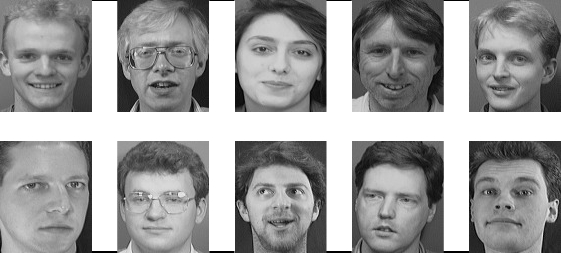
\includegraphics[scale=0.7]{Att}
    \caption{Muestra de imágenes que conforman la base de datos AT\&T}
    \label{Att}
\end{figure}
\subsection{Yale A}
Esta base de datos \cite{Yale} contiene 165 imágenes en escala de grises en formato GIF de 15 individuos. Hay 11 imágenes por sujeto, una por cada diferente expresión facial o cambio de iluminación: iluminación central , con gafas, feliz, iluminación izquierda, sin gafas ,expresión normal , iluminación derecha , triste , somnoliento , sorprendido , y guiño. Algunas de estas configuraciones pueden apreciarse en la imagen \ref{Yale}
\begin{figure}[h]
	\center
	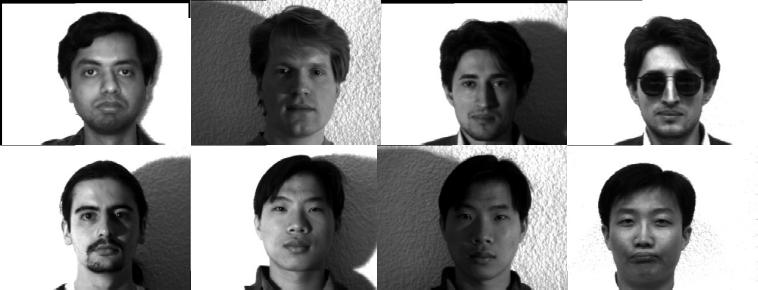
\includegraphics[scale=0.55]{Yale}
    \caption{Muestra de imágenes que conforman la base de datos Yale A}
    \label{Yale}
\end{figure}
\subsection{Georgia Tech}
La base de datos \cite{Georgia} contiene imágenes de 50 personas y se almacena en formato JPEG. Para cada individuo, hay 15 imágenes a color capturadas entre el 06/01/99 y el 15/11/99. La mayoría de las imágenes fueron tomadas en dos sesiones diferentes para tener en cuenta las variaciones en las condiciones de iluminación, la expresión facial y la apariencia. Además de esto, los rostros fueron capturados en diferentes escalas y orientaciones.

Esta base de datos a diferencia de las dos descritas anteriormente es especialmente desafiante por que no es normalizada ni recortada y como se puede observar en la Figura \ref{Georgia} donde el proceso de adquisición es más informal.
\begin{figure}[h]
	\centering
	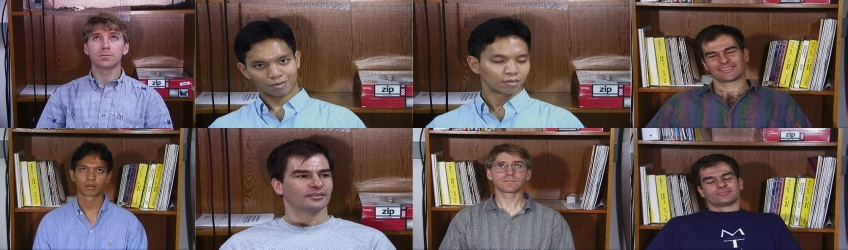
\includegraphics[scale=0.5]{Georgia}
    \caption{Muestra de imágenes que conforman la base de datos Georgia Tech}
    \label{Georgia}
\end{figure}
\subsection{Base de datos generadas a partir de imágenes de cámara de vigilancia}
\label{scc:BDCamara}
Se produjo una base de datos de una cámara de seguridad enfocando la escena vista en la Figura \ref{im:Escena}, con el objetivo de tener un referente de prueba lo mas cercano a la realidad.

La base de datos consiste en 24 sujetos con 8 imágenes cada uno separadas en dos grupos mañana y medio día para probar la variaciones en iluminación, en la Figura \ref{camara} podemos ver una muestra de la base de datos.
\begin{figure}[h]
	\centering
	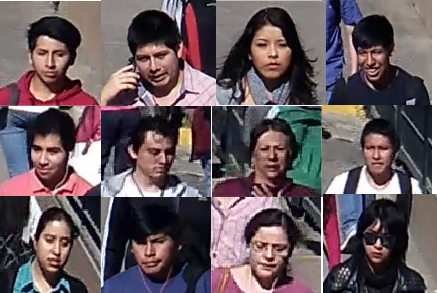
\includegraphics[scale=0.7]{camara}
    \caption{Muestra de imágenes que conforman la base de datos obtenida a partir de una cámara de seguridad}
    \label{camara}
\end{figure}

\section{Método de experimentación}\label{scc:MetdoEx}
Como método de experimentación aplicamos un proceso en cada base de datos que consiste en dividir las imágenes de cada individuo en grupos de 3 a 4 imágenes por sujeto, dependiendo de la base de datos y cada grupo fue usado como entrenamiento mientras el resto es usado como prueba. Este proceso se repite hasta que todos los grupos hayan sido usados como entrenamiento, siendo la cifra final el promedio de los resultados de cada grupo.

\begin{figure}[h]
	\centering
	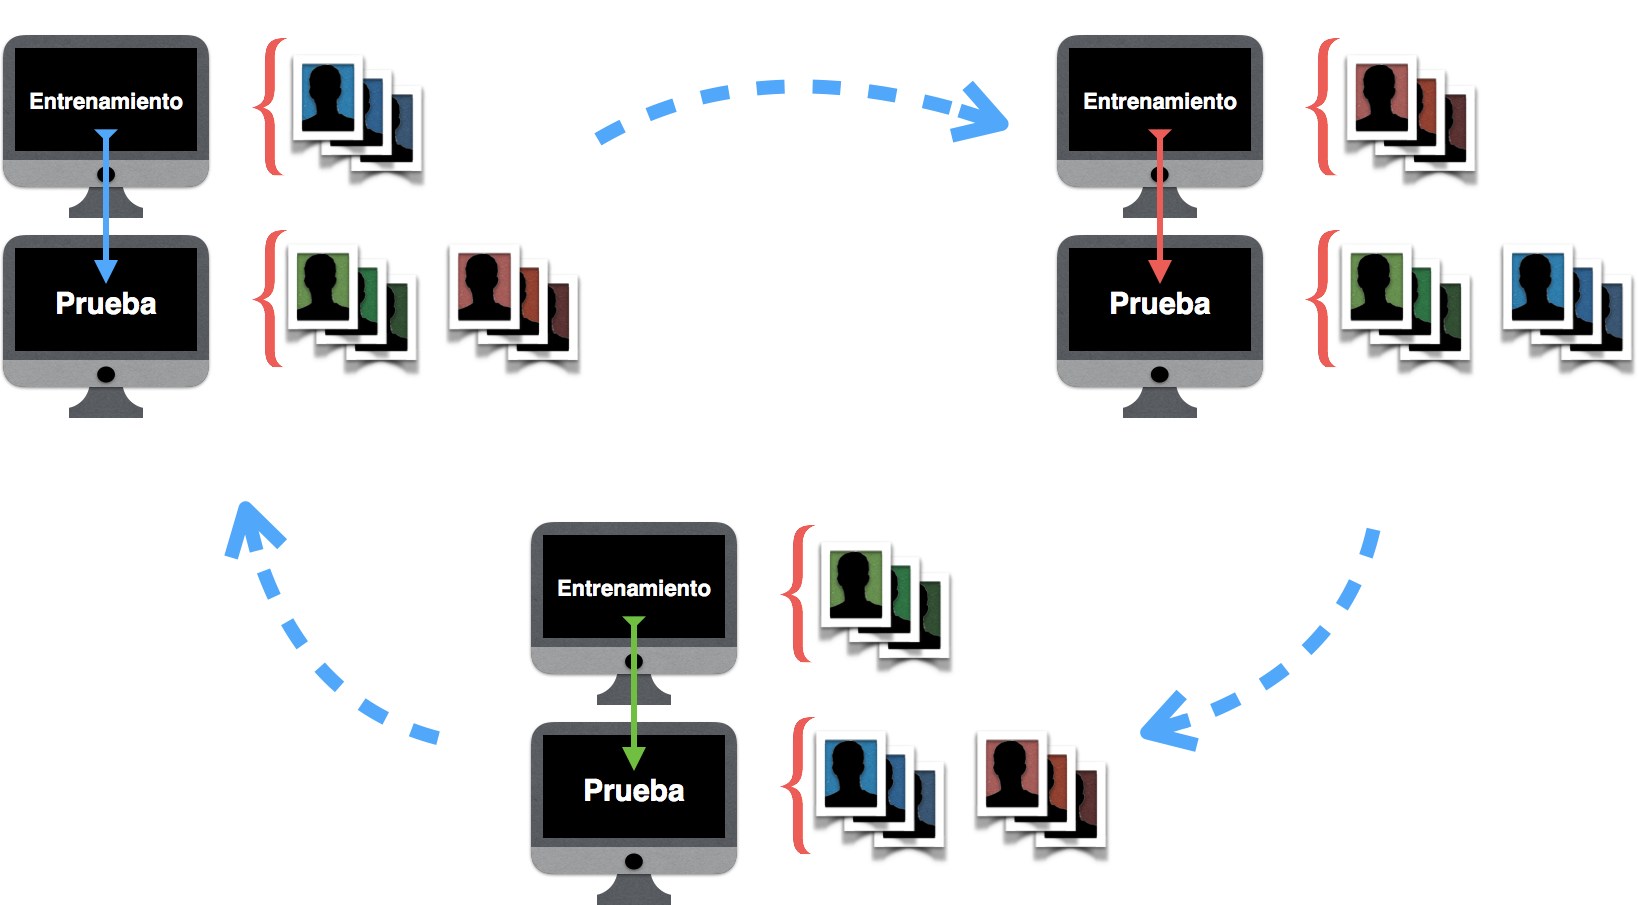
\includegraphics[scale=0.25]{MetodoExp}
    \caption{Muestra del proceso de experimentación, donde las imágenes se dividen por grupos y todos los grupos rotan hasta que todas las combinaciones de prueba y entrenamiento sean probadas}
    \label{metodo}
\end{figure}

La razón para la elección de grupos de entrenamiento tan reducidos es poder acercarnos al escenario de vídeo vigilancia donde en raras ocasiones se cuenta con varias imágenes de los sujetos a identificar.

A continuación se realiza una comparativa del método de reconocimiento usado en la propuesta y otros métodos extraídos del estado del arte.

\section{Comparación de \ac{EBGM} con métodos holísticos}\label{scc:Comparacion}
Se realizó una comparación de \ac{EBGM} con otros métodos de reconocimiento holísticos usados en la literatura como; \ac{PCA}\cite{turk1991eigenfaces}, \ac{KFA}\cite{yang2002kernel} y \ac{LDA}\cite{zhao1999subspace}, todos ellos implementados en matlab por The PhD Toolbox \cite{struc2012phd} para demostrar el rendimiento de estos algoritmos en varias situaciones. Esta comparación se realizo con las tres primeras bases de datos para establecer una diferencia entre el método escogido en la propuesta y otros métodos del estado del arte.

\begin{table}[h]
\centering
\caption{Resultados de algoritmos de reconocimiento con bases de datos ATT, Yale A y Georgia}
\label{Tcomparacion}
\begin{tabular}{|l|l|l|l|l}
\cline{1-4}
              & \textbf{ATT/ORL} & \textbf{YALE A} & \textbf{Georgia} &  \\ \cline{1-4}
\textbf{PCA}  & 88.03\%          & 88.18\%         & 76.84\%          &  \\ \cline{1-4}
\textbf{KFA}  & 87.78\%          & 91.72\%         & 75.03\%          &  \\ \cline{1-4}
\textbf{LDA}  & 86.02\%          & 90.21\%         & 75.50\%          &  \\ \cline{1-4}
\textbf{EBGM} & 91.43\%          & 97.94\%         & 77.80\%          &  \\ \cline{1-4}
\end{tabular}
\end{table}
Como se puede apreciar en el Cuadro \ref{Tcomparacion} y mejor aun en la Figura \ref{Fcomparacion}. \ac{EBGM} tiene una tasa de aciertos igual o en algunos casos mejor que los demás métodos comparados. En ninguna de las pruebas realizadas con las tres bases de datos \ac{EBGM} cae por debajo de la tasa de aciertos promedio, esta es una de las razones por la cual se elige a \ac{EBGM} como el método de reconocimiento de rostros en el cual se centra el trabajo de esta tesis.

\begin{figure}[h]
\center
	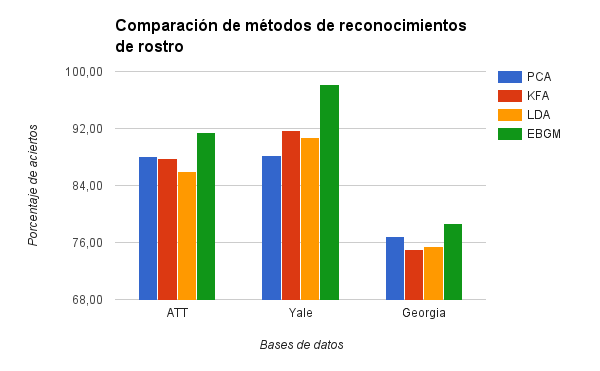
\includegraphics[scale=0.8]{Comparativa}
    \caption{Comparación de \ac{EBGM} con otros algoritmos, la escala empieza en 68,00 para que pueda apreciarse las diferencias entre los métodos}
    \label{Fcomparacion}
\end{figure}
\section{Evaluación paramétrica de \ac{EBGM}}

El método elegido para el proceso de reconocimiento de rostros es \ac{EBGM}, este ha sido elegido por sus resultado en la comparativa realizada en la Sección \ref{scc:Comparacion}, también por ser un método que es considerado biométrico por lo expuesto en el Capítulo \ref{chap:Conceptos}.

Parte de las contribuciones de este trabajo de tesis consiste en una evaluación de parámetros de \ac{EBGM} para poder incrementar la tasa de aciertos, entiéndase como tasa de acierto al porcentaje respecto a los verdaderos positivos. Finalmente probar el resultado en un ambiente de vídeo vigilancia.

\begin{figure}[h]
\center
	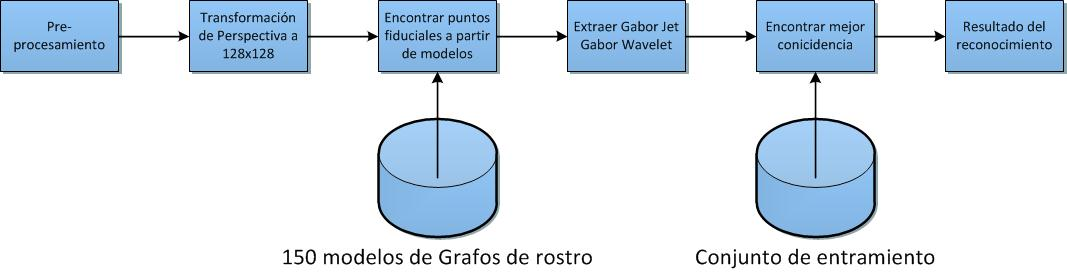
\includegraphics[scale=0.65]{EBGMproccess}
    \caption{Curso de procesos que forman parte del reconocimiento de rostros en \ac{EBGM}}
    \label{im:parametos}
\end{figure}

Se puede observar el curso normal de \ac{EBGM} en la Figura \ref{im:parametos}, y las evaluaciones que se plantean son las siguientes:

\subsection{Incrementar la cantidad de modelos}
En el trabajo de \cite{bolme2003elastic} se usa 70 modelos de rostros de la base de datos FERET gray, el numero de modelos es el mismo que se usa en el trabajo de \cite{wiskott1997face} al que hace referencia.

Para la creación de los modelos se usó la nueva versión de FERET llamada FERET COLOR y se ha elegido nuevas imágenes aleatoriamente para extraer manualmente las coordenadas de los puntos fiduciales, así mismo se ha incrementado el numero de modelos a 150 con el fin de probar si dicho incremento tiene una relación directa con la tasa de aciertos.

\begin{table}[h]
\centering
\caption{Resultado aciertos con incremento de modelos en \ac{EBGM}}
\label{ta:ModelInc}
\begin{tabular}{|c|c|c|c|}
\hline 
                     & \textbf{AT\&T/ORL} & \textbf{Yale A} & \textbf{Georgia} \\ \hline
\textbf{\ac{EBGM} original}  & 91.43\%            & 97.94\%         & 77.80\%          \\ \hline
\textbf{150 Modelos}         & 91.43\%            & 98.21\%         & 78.73\%          \\ \hline
\end{tabular}
\end{table}

Como se puede observar en el Cuadro \ref{ta:ModelInc} existe una mejora en los aciertos, no obstante un incremento en el numero de modelos modelos no implica una mejora proporcional en la tasa de aciertos, lo cual indica que existe un punto en que la cantidad de modelos es suficiente para realizar una estimación precisa.

\subsection{Modificar la función de similitud} 
Usando como base el trabajo de \cite{bolme2003elastic}, en este trabajo se tiene como parte de sus conclusiones y recomendaciones la modificación de la función de similitud con la que se compara los Face Graph que son las representaciones de un rostros en dicho algoritmo.

La modificación que se sugiere investigar es la de añadir pesos a cada punto fiducial que se compara, ya que se puede concluir que no todos los puntos de un rostros son igualmente importantes para realizar un reconocimiento. 

Un ejemplo, es que los puntos del contorno del rostro o el cabello pueden ser menos importantes que los puntos de los ojos o la nariz, así que se añade un vector de pesos a la función de similitud descrita en la ecuación \ref{FaceGraphSimiFunc} y \ref{GaborJetSimiFunc} y probamos varias combinaciones empíricas bajo el concepto que la información con mayor relevancia se encuentra en la boca, nariz y ojos .
\begin{equation}
\label{FaceGraphSimiFuncW}
L_{jet}(G,G',W)=\frac{1}{N}\sum_{i=0}^{N}S(J_{i},J'_{i},w_{i})
\end{equation}
\begin{equation}
\label{GaborJetSimiFuncW}
S(J,J',w)=w*\frac{\sum_{j=1}^{N}a_j a'_jcos(\phi_j-\phi'_j)}{\sqrt{\sum_{j=1}^{N}a_j^2 \sum_{j=1}^{N}{a'}_j^2}}
\end{equation}

En las Ecuaciones \ref{FaceGraphSimiFuncW} y \ref{GaborJetSimiFuncW} podemos observar la adición de un vector $W$ de tamaño $N$ con elementos $w$, lo que permite dar una valoración diferente a cada punto fiducial.

\begin{table}[h]
\centering
\caption{Tabla de distribución de pesos propuesta}
\label{ta:distPuntos}
\begin{tabular}{|l|c|c|c|c|}
\hline
\textbf{Área}                      & \multicolumn{1}{l|}{\textbf{Nro puntos}} & \multicolumn{1}{l|}{\textbf{Conf. 1}} & \multicolumn{1}{l|}{\textbf{Conf. 2}} & \multicolumn{1}{l|}{\textbf{Conf. 3}} \\ \hline
\textbf{Ojos y puente de la nariz} & 3                                        & 20\%                                  & 50\%                                  & 15\%                                  \\ \hline
\textbf{Cejas}                     & 6                                        & 20\%                                  & 10\%                                  & 15\%                                  \\ \hline
\textbf{Nariz}                     & 4                                        & 20\%                                  & 20\%                                  & 20\%                                  \\ \hline
\textbf{Boca}                      & 4                                        & 20\%                                  & 10\%                                  & 25\%                                  \\ \hline
\textbf{Bordes de la cabeza}       & 5                                        & 10\%                                  & 5\%                                   & 5\%                                   \\ \hline
\textbf{Barbilla y quijada}        & 3                                        & 10\%                                  & 5\%                                   & 20\%                                  \\ \hline
\end{tabular}
\end{table}

En el Cuadro \ref{ta:distPuntos} se observa la agrupaciones que se realizan a los puntos fiduciales y las distribuciones mostradas como porcentajes, donde se le da importancia a áreas que se ubican en el centro del rostro, en el cuadro \ref{ta:Pesos} se puede ver su correspondencia en valores numéricos para la conformación del vector $W$ usado en la Ecuación \ref{FaceGraphSimiFuncW}.

\begin{table}[h]
\centering
\caption{Valores del vector W de pesos derivado del Cuadro \ref{ta:distPuntos}}
\label{ta:Pesos}
\resizebox{\textwidth}{!}{
\begin{tabular}{|l|c|c|c|}
\hline
\textbf{Puntos Fiduciales}                    & \multicolumn{1}{l|}{\textbf{1ra Config}} & \multicolumn{1}{l|}{\textbf{2da Config}} & \multicolumn{1}{l|}{\textbf{3ra Config}} \\ \hline
\textbf{ojo izquierdo}                         & 0.07                                      & 0.07                                     & 0.05                                                                         \\ \hline
\textbf{ojo derecho}                           & 0.07                                      & 0.07                                     & 0.05                                                                         \\ \hline
\textbf{puente de la nariz}                    & 0.06                                      & 0.07                                     & 0.05                                                                         \\ \hline
\textbf{pico ceja derecha}                     & 0.03                                      & 0.025                                    & 0.025                                                                        \\ \hline
\textbf{pico ceja izquierda}                   & 0.03                                      & 0.025                                    & 0.025                                                                        \\ \hline
\textbf{interior ceja derecha}                 & 0.04                                      & 0.025                                    & 0.025                                                                        \\ \hline
\textbf{interior ceja izquierda}               & 0.04                                      & 0.025                                    & 0.025                                                                        \\ \hline
\textbf{exterior ceja derecha}                 & 0.03                                      & 0.025                                    & 0.025                                                                        \\ \hline
\textbf{exterior ceja derecha}                 & 0.03                                      & 0.025                                    & 0.025                                                                        \\ \hline
\textbf{punta de la nariz}                     & 0.05                                      & 0.08                                     & 0.05                                                                         \\ \hline
\textbf{centro base de la nariz}               & 0.05                                      & 0.07                                     & 0.05                                                                         \\ \hline
\textbf{base derecha de la nariz}              & 0.05                                      & 0.07                                     & 0.05                                                                         \\ \hline
\textbf{base izquierda de la nariz}            & 0.05                                      & 0.07                                     & 0.05                                                                         \\ \hline
\textbf{parte central superior de la boca}     & 0.05                                      & 0.0375                                   & 0.0625                                                                       \\ \hline
\textbf{parte central inferior de la boca}     & 0.05                                      & 0.0375                                   & 0.0625                                                                       \\ \hline
\textbf{esquina izquierda de la boca}          & 0.05                                      & 0.0375                                   & 0.0625                                                                       \\ \hline
\textbf{esquina derecha de la boca}            & 0.05                                      & 0.0375                                   & 0.0625                                                                       \\ \hline
\textbf{parte central superior de la cabeza}   & 0.02                                      & 0.02                                     & 0.01                                                                         \\ \hline
\textbf{parte izquierda superior de la cabeza} & 0.02                                      & 0.02                                     & 0.01                                                                         \\ \hline
\textbf{parte derecha superior de la cabeza}   & 0.02                                      & 0.02                                     & 0.01                                                                         \\ \hline
\textbf{borde izquierdo de la cara}            & 0.02                                      & 0.02                                     & 0.01                                                                         \\ \hline
\textbf{borde derecho de la cara}              & 0.02                                      & 0.02                                     & 0.01                                                                         \\ \hline
\textbf{centro de la barbilla}                 & 0.04                                      & 0.04                                     & 0.06                                                                         \\ \hline
\textbf{parte izquierda de la quijada}         & 0.03                                      & 0.03                                     & 0.07                                                                         \\ \hline
\textbf{parte derecha de la quijada}           & 0.03                                      & 0.03                                     & 0.07                                                                         \\ \hline
\end{tabular}
}
\end{table}

En el Cuadro \ref{ta:ResultadosPesos} se observan los resultados de las configuraciones propuestas para modificación la función de similitud de \ac{EBGM}, en la figura \ref{im:ResultadoPesos} vemos que la primera configuración ofrece una mejora de 2\% en la base de datos Georgia y mantiene el rendimiento en el resto de las base de datos. Esta configuración distribuye los pesos uniformemente a todas las áreas del centro del rostro en detrimento de los bordes como son la barbilla y la quijada.

\begin{table}[h]
\centering
\caption{Resultados de adición de pesos \ac{EBGM}}
\label{ta:ResultadosPesos}
\begin{tabular}{|l|l|l|l|}
\hline
\textbf{Propuestas}                     & \textbf{AT\& T} & \textbf{Yale} & \textbf{Georgia} \\ \hline
\textbf{\ac{EBGM} sin cambios}             & 91.43\%      & 97.94\%       & 77.80\%          \\ \hline
\textbf{Primera configuración de pesos} & 91.67\%      & 97.58\%       & 80.43\%          \\ \hline
\textbf{Segunda configuración de pesos} & 91.15\%      & 97.86\%       & 79.40\%          \\ \hline
\textbf{Tercera configuración de pesos} & 90.16\%      & 96.71\%       & 76.70\%          \\ \hline
\end{tabular}
\end{table}

En el resto de las configuraciones se observan resultados variados donde se presentan mejoras del 1\% en las tres bases de datos con excepción de la tercera configuración donde se le resta importancia a los ojos, para probar la importancia del centro del rostro como fuente de información.

\begin{figure}[ht]
	\centering
	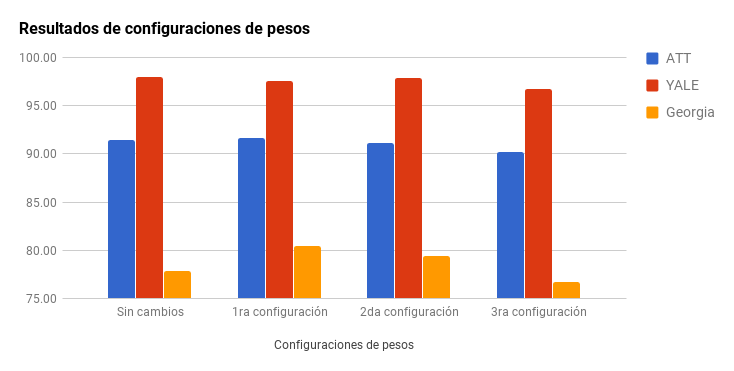
\includegraphics[scale=0.6]{ResultadoPesos}
    \caption{Comparación entre las configuraciones propuestas para los pesos en la función de similitud de \ac{EBGM}}
    \label{im:ResultadoPesos}
\end{figure}

\subsection{Incrementar la cantidad de imágenes de entrenamiento a través de transformaciones de perspectiva} 
Una de las restricciones más grandes que conlleva el reconocimiento de rostros en vídeo vigilancia, es el hecho de que en muchos sistema de vigilancia no se cuenta con varias imágenes por sujeto para realizar un entrenamiento adecuado. En muchos casos solo se cuenta con una imagen, ya puede ser de un carnet o una fotografía de perfil y en varios casos son imágenes que no están al día. 

Por ello se plantea crear más imágenes de entrenamiento a partir de una sola imagen a través de varias transformaciones de perspectiva para probar si con una imagen frontal podemos crear imágenes de rostros que parezcan mirar a otros sentidos y así poder aumentar el numero de entrenamiento y con ello el porcentaje de aciertos.

\begin{figure}[h]
	\centering
	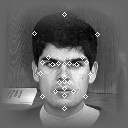
\includegraphics[scale=1]{trans_original}
    \caption{Imagen de entrenamiento original}
\end{figure}

Para lograr ello generamos una matriz de transformación en 3D donde realizamos las rotaciones necesarias en el eje Z para crear la ilusión de cambio de pose, después realizamos un conversión a un matriz de transformación 2D y la aplicamos a la imagen. Los resultados de dicha transformación se pueden apreciar en la Figura \ref{im:Transformacion}.

\begin{figure}[h]
	\centering
	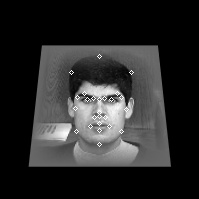
\includegraphics[scale=0.6]{trans1}
    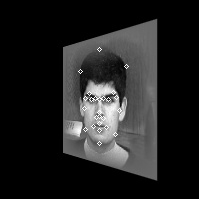
\includegraphics[scale=0.6]{trans2}
    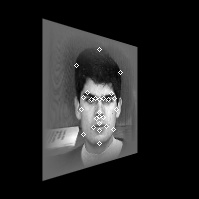
\includegraphics[scale=0.6]{trans3}
    \caption{Resultados de las transformaciones de perspectiva}
    \label{im:Transformacion}
\end{figure}

En las pruebas hechas a \ac{EBGM}, no se muestra ningún cambio y en los resultados experimentales. el uso de las trasformaciones no ayudan a mejorar la tasa de aciertos pero tampoco la empeoran. En ningún caso una imagen generada por la transformación de perspectiva es elegida como resultado del proceso de reconocimiento.

\subsection{Ajuste de tamaño a máscaras de Gabor}
La Ecuación \ref{GaborWavelet} define el Gabor Wavelet que se usa para crear máscaras de Gabor. Con esta ecuación podemos crear varios tamaños de máscaras, donde la configuración original es $N \in \left\{25, 37, 51, 71, 101 \right\}$. En conjunción al resto de parámetros explicados en la Sección \ref{sscc:GaborWavelet} se obtienen 80 configuraciones de Gabor Wavelet y siendo efectivas 40 máscaras por punto fiducial, debido a que existe una mascara que extrae la parte imaginara y otra la parte real del Wavelet.

La propuesta de modificación plantea el cambio del tamaño de las Gabor Wavelet, debido a que tamaños de 71 y 101 son demasiado grandes teniendo en cuenta que la imagen a convolucionar es de $128 \times 128$ y el tamaño efectivo del rostro es aun menor siendo los tamaños propuestos $N \in \left\{13, 19, 25, 35, 51 \right\}$ los resultados pueden observarse en el Cuadro

\begin{table}[h]
\centering
\caption{Resultados de pruebas en tamaños de mascaras de Gabor }
\label{ta:ResultadosMascaras}
\begin{tabular}{|l|c|c|c|}
\hline
\textbf{}                                         & \multicolumn{1}{l|}{\textbf{AT\&T}} & \multicolumn{1}{l|}{\textbf{Yale}} & \multicolumn{1}{l|}{\textbf{Georgia}} \\ \hline
\textbf{Sin cambios}                              & 91.43\%                             & 97.94\%                            & 77.80\%                               \\ \hline
\textbf{Propuesta de mascaras de Gabor} & 93.18\%                             & 97.58\%                            & 79.43\%                               \\ \hline
\end{tabular}
\end{table}

Se observa mejoras de 2\% en las bases de datos AT\&T y Georgia, mientras que en Yale mantiene el porcentaje de aciertos. Un efecto a parte de la mejora en el acierto es que al tener un tamaño de mascaras menor el tiempo en convoluciones también se disminuye.
\section{Evaluaciones en el \textit{pipeline} de reconocimiento}
Como parte de la propuesta es necesario encontrar un método de validación para confirmar las detecciones de rostros proporcionadas por el algoritmo de Viola-Jones, en esta sección se muestran resultados sobre las opciones exploradas para afrontar este problema

\subsection{Evaluación del detector de Viola-Jones para detección de ojos}\label{sscc:DectOjos}
Para poder usar \ac{EBGM} tal como se presenta en \cite{bolme2003elastic} y \cite{wiskott1997face} en un \textit{pipeline} de vídeo vigilancia es necesario proporcionar las coordenadas de los ojos.

Para ello se necesita establecer un proceso o una forma de detección de ojos con una gran robustez, ya que un error en la detección de ojos resulta en un fallo de todo el proceso de reconocimiento

Como parte de este trabajo se realizo pruebas de un detector de Viola-Jones entrenado para detectar ojos como opción para encontrar coordenadas de ojos y empezar el proceso de reconocimiento. Para ello se probó el Algoritmo \ref{alg:DetecOjos}.

\begin{algorithm}
\label{alg:DetecOjos}
\var{face} $\gets$ rostro detectado por un detector de rostros\;
\var{eyes} $\gets$ lista de ojos detectados en \var{face}\;
\For{\var{i}  $\gets$ 0, \var{i}< tamaño de \var{eyes}}
{
    \If{la posición de \var{$eyes_[i]$} no se encuentra en la región superior central de \var{face}}
    {
    	descartar \var{$eyes_[i]$} de \var{eyes}\;
    }
}
\var{region} $\gets$ dividir la región superior central de \var{face} en cuatro pares de sub-regiones \;
agrupar todos los ojos detectados en \var{eyes} segun su posicion dentro de \var{region}\;
\For{cada \var{region}}
{
	calcular el punto promedio a partir todos los \textit{eyes} en  \textit{region}\;
}
Elegir el par de puntos perteneciente al par de \textit{region} según la mayor cantidad de puntos que posee\;
\caption{Proceso de detección de ojos en rostro para \ac{EBGM}}
\end{algorithm}

\begin{figure}[h]
	\centering
	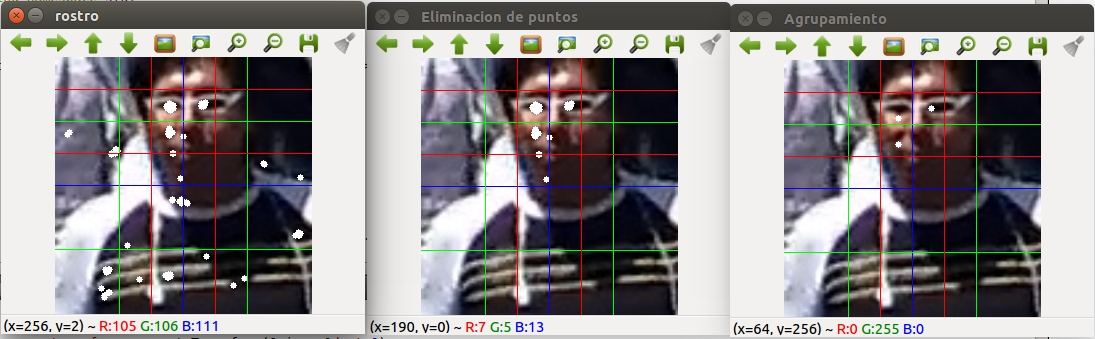
\includegraphics[scale=0.35]{OjosViolaJones}
    \caption{Ejemplo de proceso de detección de ojos Nro 1}
    \label{im:HaarOjos1}
\end{figure}

Como se puede observar en las Figuras \ref{im:HaarOjos1} y \ref{im:HaarOjos2} el proceso que propone el algoritmo \ref{alg:DetecOjos} ofrece resultados variados, el motivo de ello es la naturaleza del algoritmo de Viola-Jones, los ojos poseen menos variaciones de sombras si se lo compara con un rostro y ademas el calculo imagen integral es dependiente a la iluminación de la imagen.

\begin{figure}[h]
	\centering
    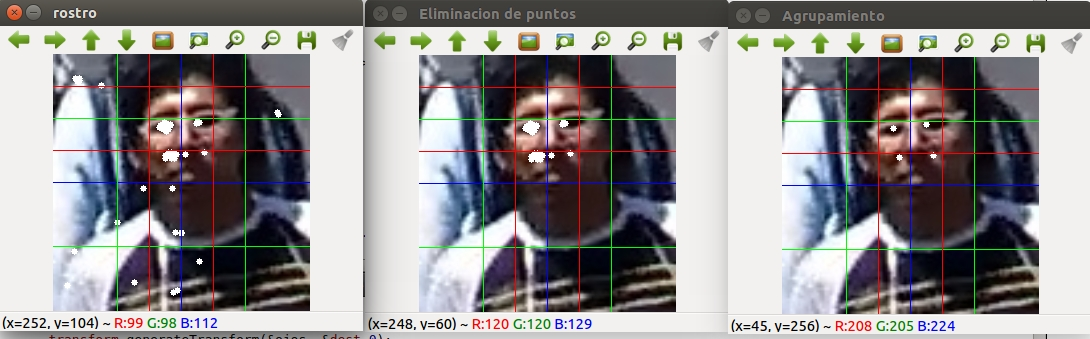
\includegraphics[scale=0.35]{OjosViolaJones2}
    \caption{Ejemplo de proceso de detección de ojos Nro 2}
    \label{im:HaarOjos2}
\end{figure}

\subsection{Validación de detecciones mediante color de piel}
Se probó como método de validación de las detecciones proporcionadas por Viola-Jones, el uso de un método de confirmación a través de detectores de color de piel sel cual se detalla en el algoritmo \ref{alg:ColorPiel}.

\begin{algorithm}[h]
\label{alg:ColorPiel}
\var{face} $\gets$ rostro detectado\;
\var{imageHSV} $\gets$ convertir \var{face} a espacio de color HSV\;
\var{binaryImage} $\gets$ binarizar imagen bajo un threshold de 70 en el canal Hue de \var{imageHSV}\;
\var{count} $\gets$ contar pixeles blancos de \var{binaryImage}\;
\eIf{\var{count}> al 50\% del total de pixeles de \var{face}}
{
	validar \var{face} como imagen de un rostros\;
}
{
	descartar \var{face} como imagen de un rostros\;
}
\caption{Validación de detecciones a través de color de piel}
\end{algorithm}

Realizando pruebas en videos como se puede ver en la figura \ref{im:skinDetector}, se observan problemas de validación debido a que los colores de piel están entre 0 y 70 en canal Hue, pero también están otros colores como el naranja se encuentran en ese mismo rango debido a la variación de los otros dos canales. Así mismo todos los colores de piel humana no se encuentran agrupados en una sola región del rango de todo el canal, sobre todo colores oscuros de piel.
\begin{figure}[h]
	\centering
    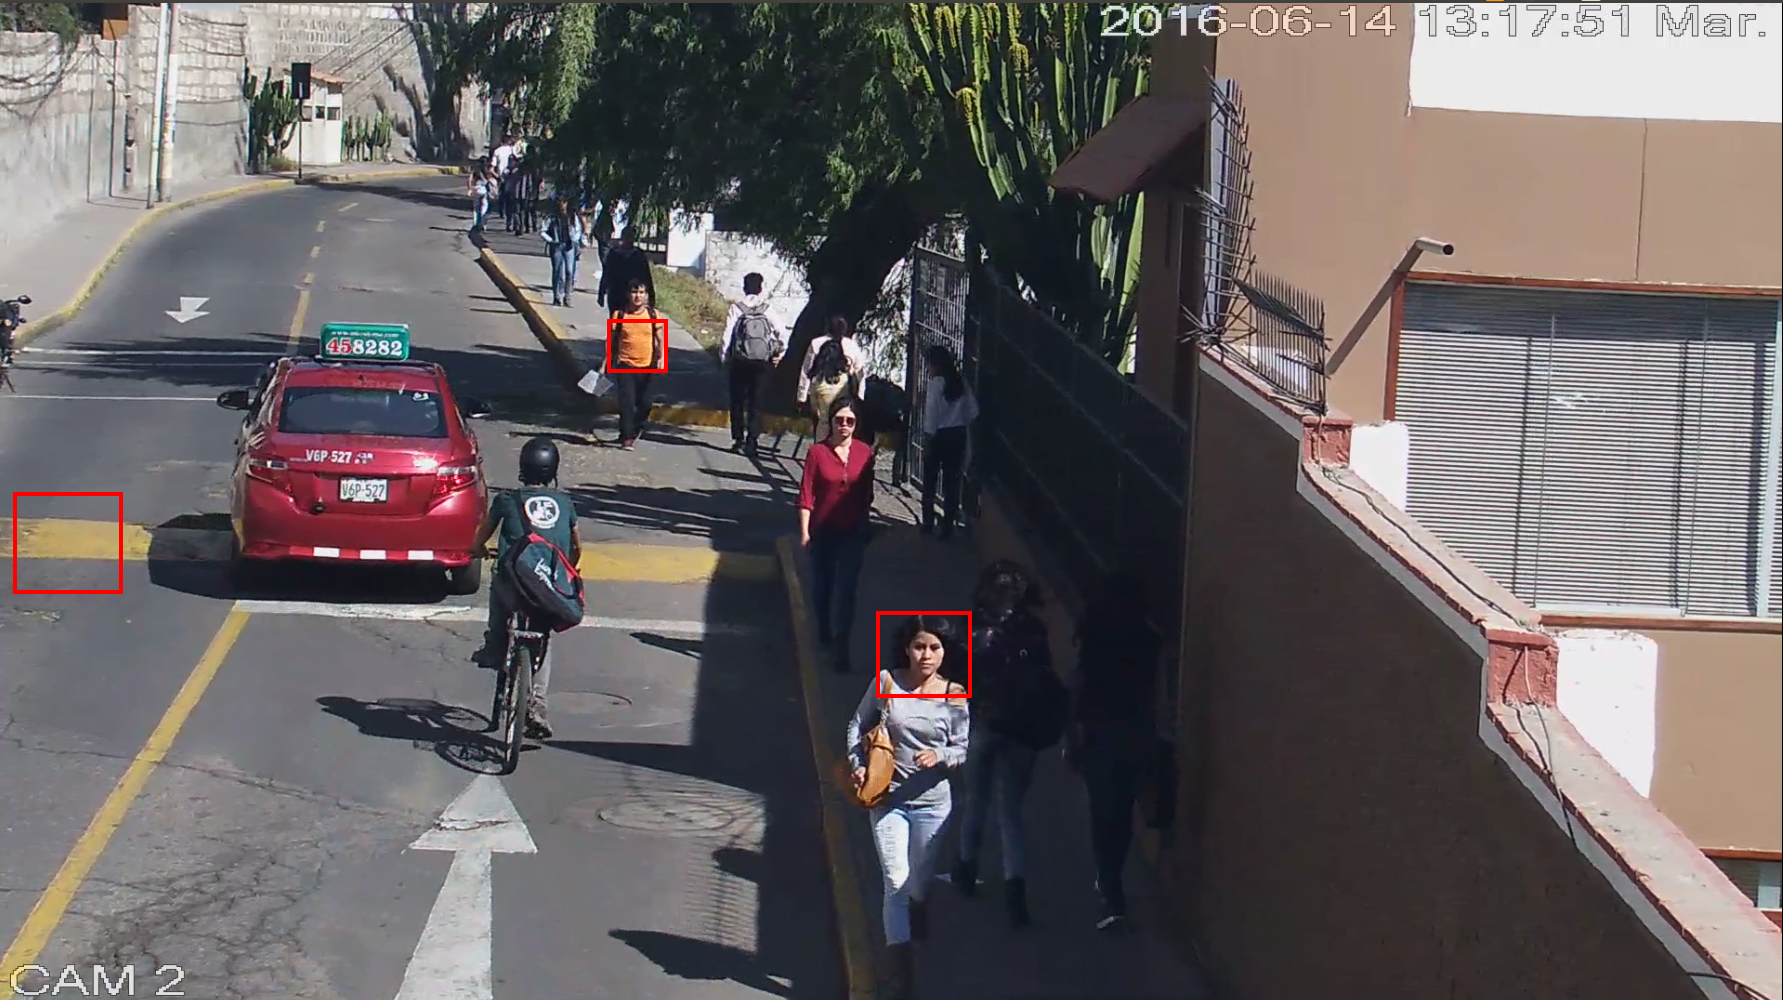
\includegraphics[scale=0.2]{SkinDetector}
    \caption{Ejemplo de falsas validaciones en colores cercanos al rojo y naranja.}
    \label{im:skinDetector}
\end{figure}

\subsection{Mejora de la iluminación en el pre-procesamiento} 
\ac{EBGM} tiene un pre-procesamiento para normalizar la información introducida, pero este pre-procesamiento solo consiste en una normalización de los valores de los pixeles de las imágenes, una transformación de tamaño a un estándar de $128 \times 128$ y la añadidura de bordes de 30 pixeles a la imagen. 
El uso de esto bordes se justifican en el trabajo de \cite{bolme2003elastic} como una forma de ayudar a que su ajuste de puntos fiduciales converja en el centro de la imagen y no tienda a alejarse a los borde, y como método para filtrar la información del fondo que pueda quedar después de la transformación de perspectiva aplicada.

Para cubrir esta falta de una mejora en iluminación, la propuesta explicada en la Sección \ref{scc:PropIluminacion} implica la modificación de este proceso para así volverlo más robusto a cambios de luz.

\begin{table}[h]
\centering
\caption{Resultados de la propuesta de iluminación}
\label{ta:ResultadosIluminacion}
\begin{tabular}{|l|c|c|c|}
\hline
\textbf{}                           & \multicolumn{1}{l|}{\textbf{AT\&T}} & \multicolumn{1}{l|}{\textbf{Yale}} & \multicolumn{1}{l|}{\textbf{Georgia}} \\ \hline
\textbf{\ac{EBGM} sin cambios}                & 91.43\%                             & 97.94\%                            & 77.80\%                               \\ \hline
\textbf{Ecualización de histograma} & 92.78\%                             & 96.67\%                            & 79.13\%                               \\ \hline
\textbf{Propuesta de iluminación}   & 92.82\%                             & 98.53\%                            & 78.93\%                               \\ \hline
\end{tabular}
\end{table}

La unión de procesos expuesta en la ecuación \ref{f_normaliza} es comparada con el algoritmo sin cambios y con la ecualización de histograma, los resultados se pueden observar en el Cuadro \ref{ta:ResultadosIluminacion} y la Figura \ref{im:ResultadoIluminacion} donde existen mejoras del 1\% en comparación al algoritmo original y en la base de datos Yale donde la presencia de grandes contrastes afectan el reconocimiento, la ecualización de histograma obtiene un resultado inferior al algoritmo original, mientras que la propuesta logra una mejora de 1\%.
%como que tenemos que agregar algo mas

\begin{figure}[h]
    \centering
    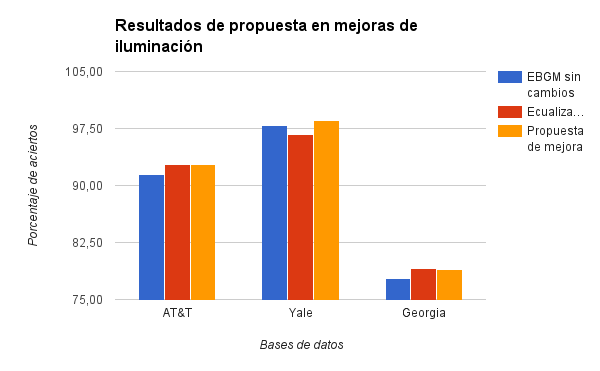
\includegraphics[scale=0.7]{ResultadoIluminacion}
    \caption{Comparación entre propuesta, ecualización de histograma y  \ac{EBGM}}
    \label{im:ResultadoIluminacion}
\end{figure}

\subsection{Tracking de rostros}
Se hizo pruebas con el algoritmo de Camshift como método de \textit{tracking}, al igual que el detector de piel presenta los problemas relacionados al color, ya que se basa en información de color proporcionada por la región inicial y en la siguiente escena busca la misma  proporción de información en regiones cercanas.

\begin{figure}[ht]
	\centering
	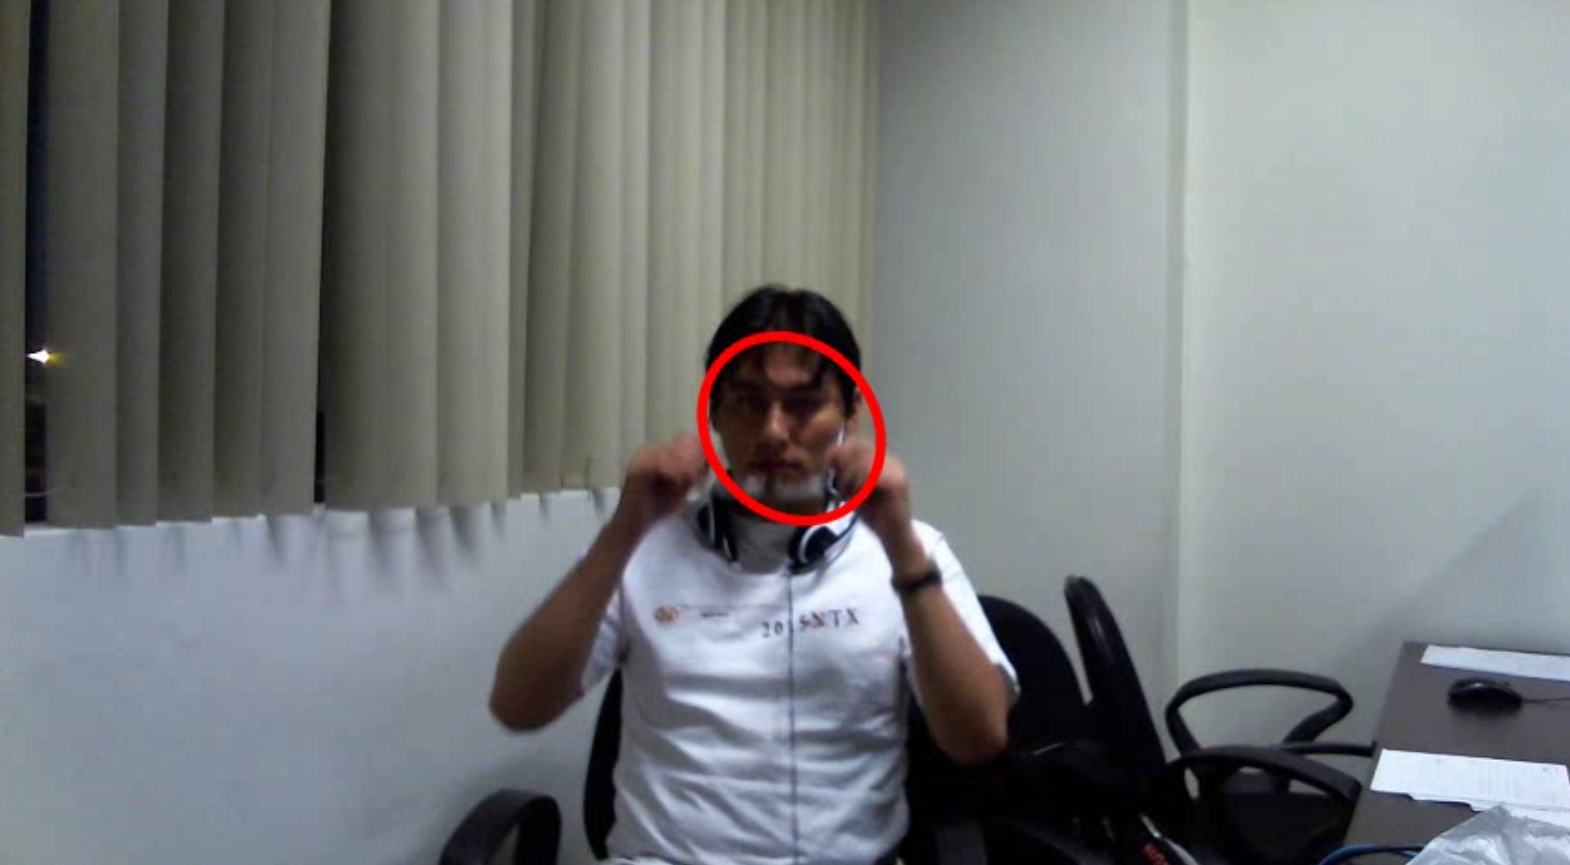
\includegraphics[scale=0.25]{CamShift1}
    \caption{Ejemplo de tracking usando Camshift}
    \label{im:CamShift1}
\end{figure}

En las figuras \ref{im:CamShift1} y \ref{im:CamShift2} se puede observar otro comportamiento de camshift, si objetos del mismo color se acercan al área de \textit{tracking}, dicha área se incrementa e incluso puede ser tomada por otro patrón de color

\begin{figure}[ht]
	\centering
	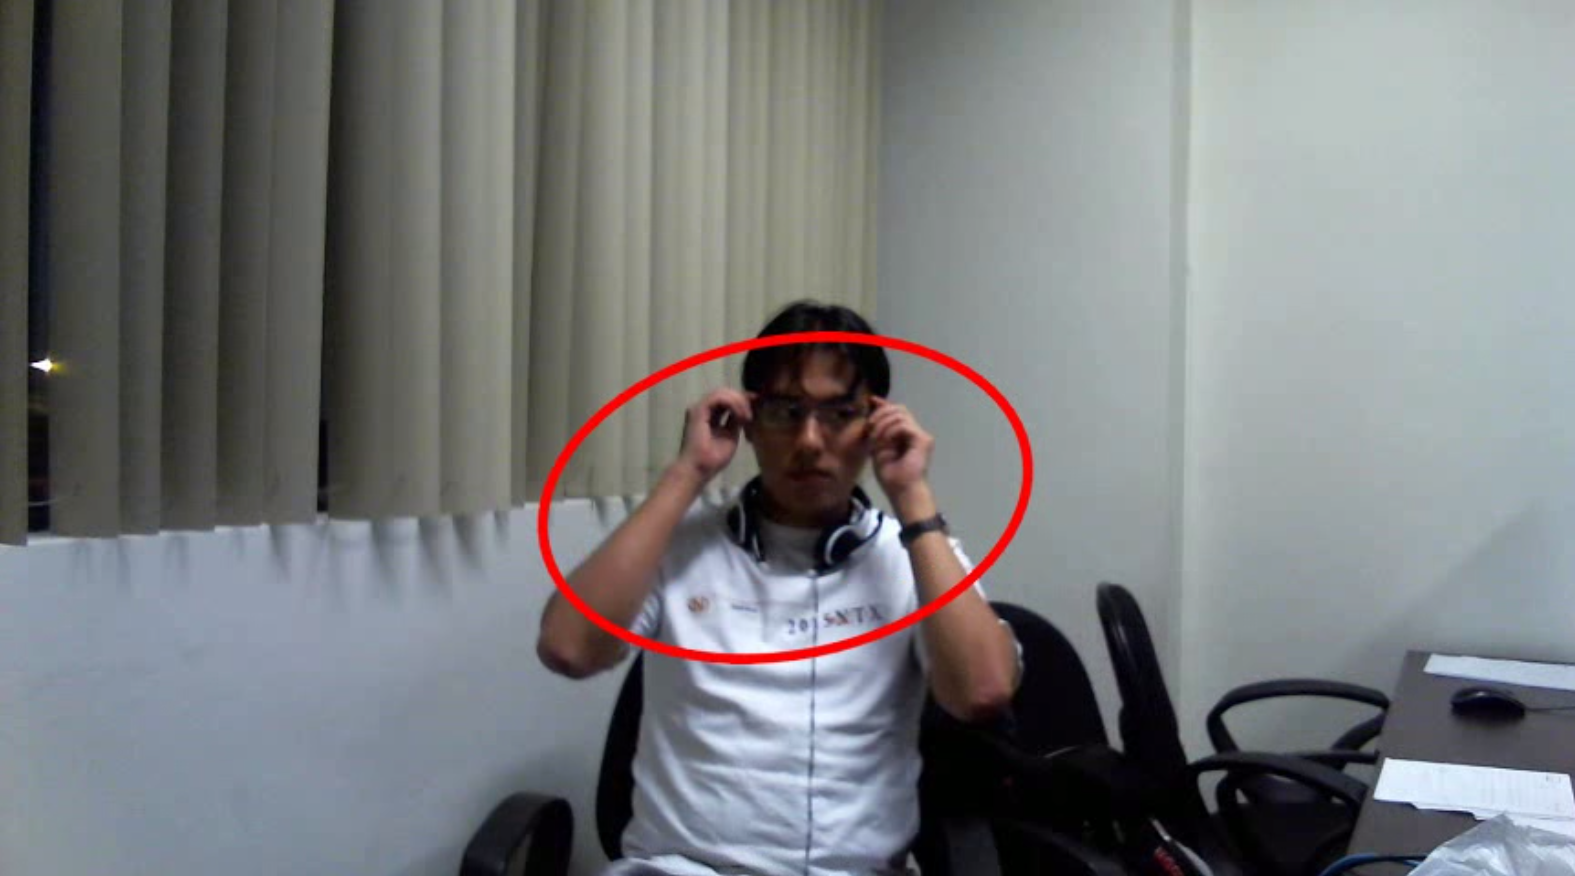
\includegraphics[scale=0.25]{CamShift2}
    \caption{Ejemplo de como el área de tracking se expande debido a áreas circundantes del mismo color}
    \label{im:CamShift2}
\end{figure}

Por las razones explicadas, se opta por usar un enfoque de \textit{tracking} a través de detecciones continuas usando el algoritmo de Viola-Jones donde errores ocasionados por los cambios de iluminación son menores que los que presenta camshift.

\subsection{Evaluar la detección de puntos fiduciales}\label{scc:ResultCLNF}
\ac{EBGM} usa modelos hechos a mano como base para encontrar puntos fiduciales, este proceso empieza con un grafo promedio generado a partir de todos los modelos, es necesario proveer las coordenadas de los ojos, a partir de esto dos punto se calcula un tercero a partir de las distancias proporcionadas por el grafo promedio y el proceso se repite a través de todos los puntos, después hace una comparación de similitud por cada punto ubicado con el mismo punto en todos los moldes, se elige la información de coordenada del molde más similar y se estima el nuevo valor del punto calculando una desviación entre el punto del grafo promedio y del obtenido a partir del modelo incluyendo el grado de similitud dando el punto final donde se extraerá las características.

\subsubsection{Comprobación entre punto manuales y puntos encontrados por \ac{EBGM}}


\ac{EBGM} depende de los modelos manuales, si no existe un modelo lo suficientemente parecido a la imagen es probable que no se realice una buena estimación de los puntos fiduciales, otro problema es que en un ambiente de vídeo se depende de un detector rostros y probablemente un detector de ojos, o uno que realice ambos trabajos lo que hace depender el resultado del reconocimiento de la correcta detección de los rostros y ojos en vídeo.

Para probar en cuanto afecta una correcta localización de puntos fiduciales se realizo la siguiente prueba: de los resultados obtenidos de la base de datos Georgia elegimos 8 sujetos con los peores resultados de aciertos y detectamos los punto fiduciales manualmente, después comparamos con el resultado si los puntos fiduciales hubiera sido localizados con los moldes.


\begin{table}[h]
\centering
\caption{Comparación de puntos fiduciales}
\label{TpuntosManuales}
\begin{tabular}{|l|c|c|c|}
\hline
\textbf{ }                                                                     & \multicolumn{1}{l|}{\textbf{3 Rostros}} & \multicolumn{1}{l|}{\textbf{2 Rostros}} & \multicolumn{1}{l|}{\textbf{1 Rostro}} \\ \hline
\textbf{\begin{tabular}[c]{@{}l@{}}Sin Cambios\\ con modelos\end{tabular}}                  & 65.75\%                                 & 66.62\%                                 & 57.14\%                                \\ \hline
\textbf{\begin{tabular}[c]{@{}l@{}}Puntos manuales \\ Entrenamiento aleatorio\end{tabular}} & 77.92\%                                 & 74.31\%                                 & 64.11\%                                \\ \hline
\textbf{\begin{tabular}[c]{@{}l@{}}Puntos manuales \\ Entrenamiento escogido\end{tabular}}  & 91.67\%                                 & 81.73\%                                 & 80.36\%                                \\ \hline
\end{tabular}
\end{table}
Como se observa en la Cuadro \ref{TpuntosManuales} tenemos la primera fila que es el resultado de \ac{EBGM} sin ningún cambio, en la segunda tenemos los resultados usando una localización manual en vez de los moldes originales y la ultima fila es el mismo resultado donde elegimos una imagen de perfil y dos imágenes  mirando a ambos lados, las columnas se refieren a la cantidad de rostro que se usa como entrenamiento. Para esta prueba se utilizó solo la base de datos Georgia debido a como muestran las pruebas anteriores esta base de datos muestra el porcentaje de aciertos más bajo. 

Como se puede ver en las columnas del Cuadro \ref{TpuntosManuales} la primera representa el método de experimentación con el cual se ha llevado a cabo todos los experimentos, Sección \ref{scc:MetdoEx}, y las dos siguientes columnas son pruebas de cuanto mas se puede reducir el entrenamiento.
Cabe resaltar que los resultados entre el algoritmo original y el uso de \ac{CLNF} con el método de experimentación de las demás pruebas es de 65.75\% y 77.92\% y cuando se escoge especialmente las imágenes de entrenamiento la tasa de aciertos aumenta a 91.67\%, por lo que se puede observar que la forma de detección de puntos fiduciales es el punto mas débil de \ac{EBGM}.

\subsubsection{Uso de \ac{CLNF} como detector de puntos fiduciales}
La propuesta de esta tesis es usar \ac{CLNF} como método de detección de puntos fiduciales en reemplazo para ello realizamos las pruebas solo en la base de datos Georgia por ser la base de datos que muestra el menor porcentaje de aciertos. En la sección anterior se probó que la localización manual es superior al método usado por el algoritmo original de \ac{EBGM}.

Para probar que la propuesta es una mejor alternativa se hizo una comparación del algoritmo sin cambios y reemplazando el proceso de detección de puntos que usa \ac{EBGM} con el algoritmo de \ac{CLNF} esta vez usando la totalidad de la base de datos Georgia, en la figura \ref{im:ResultadosPuntos} se aprecia una mejora del 1\% con respecto al algoritmo original, ademas con el uso de \ac{CLNF} se puede dar uso a \ac{EBGM} sin los problemas mencionados en la sección \ref{sscc:DectOjos} 

\begin{table}[h]
\centering
\caption{Resultado de uso de \ac{CLNF} como detector de puntos fiduciales para \ac{CLNF}}
\label{ta:ResultadosPuntos}
\begin{tabular}{|l|c|}
\hline
\textbf{}                   & \textbf{Georgia} \\ \hline
\textbf{EBGM sin cambios}   & 77.80\%          \\ \hline
\textbf{CLNF con 68 puntos} & 78.73\%          \\ \hline
\textbf{CLNF con 22 puntos} & 79.33\%          \\ \hline
\end{tabular}
\end{table}


El uso de \ac{CLNF} tal como lo propone \cite{baltrusaitis2013constrained} entrega un grupo de 68 puntos como se puede observar en la Figura \ref{im:68Landmark} mientras que \ac{EBGM} usa 25, Cuadro \ref{ta:PuntosFiduciales}, pero entre estos dos grupos no existe correspondencia para los tres puntos que se refieren a cabello. Por lo que se realiza un filtrado para solo corresponder a 22 puntos fiduciales.

\begin{figure}[h]
    \centering
    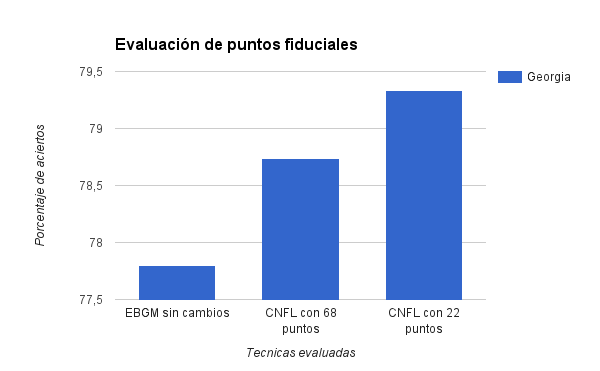
\includegraphics[scale=0.7]{ResultadosPuntos}
    \caption{Resultado de pruebas de puntos fiduciales, donde \ac{CLNF} con 22 es la propuesta final y \ac{CLNF} con 68 es el resultado sin un filtrado de puntos}
    \label{im:ResultadosPuntos}
\end{figure}

En los resultados expuestos en la tabla \ref{ta:ResultadosPuntos} y la figura \ref{im:ResultadosPuntos} se observa que después del filtrado de puntos obtenemos mejores resultado que con la totalidad de puntos entregados por\ac{CLNF}, esto se puede explicar por la eliminación de datos redundantes, gracias a ello se obtienen mejoras de 2\% con una menor cantidad de puntos a convolucionar.


\section{Prueba con base de datos de vídeo vigilancia}

La propuesta final fue probada con imágenes extraídas de una cámara de vídeo vigilancia, sección \ref{scc:BDCamara}, para ello creamos dos grupo de datos de 12 sujetos con 8 imágenes cada uno, ambos grupos obtenidos en diferentes momentos del día uno en la mañana y otro en medio día, en la escena mostrada en la figura \ref{im:Escena}.

\begin{figure}[h]
	\centering
	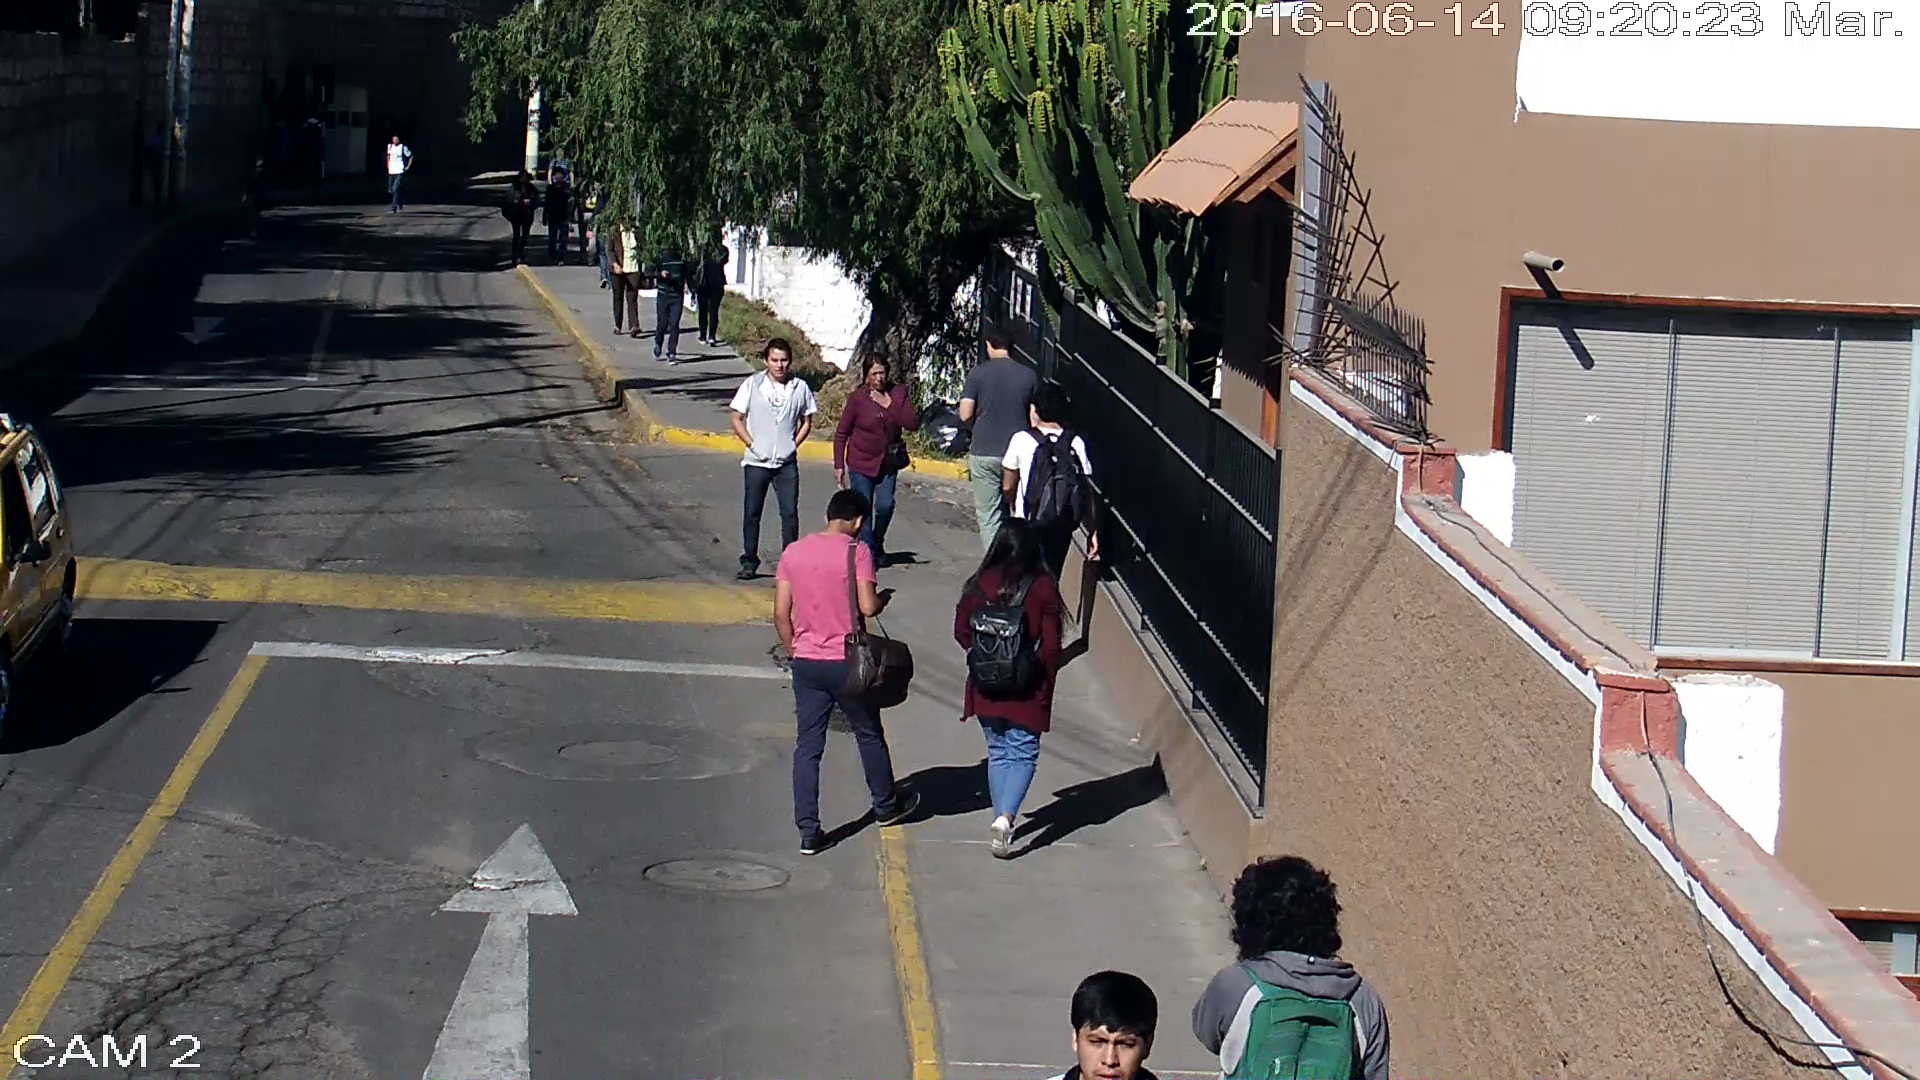
\includegraphics[scale=0.2]{Escena}
    \caption{Escena de captura de imágenes para pruebas}
    \label{im:Escena}
\end{figure}

La adquisición de datos se realizo sin la colaboración de los sujetos para que los resultados de las pruebas se acerquen lo mas posible a la realidad, a diferencia de otras bases de datos normalizadas. En la tabla \ref{ta:resultadosCLNF} podemos ver los resultados de la propuesta comparados con el algoritmo original.

\begin{table}[h]
\centering
\caption{Resultados de la propuesta en comparación a \ac{EBGM} sin cambios}
\label{ta:resultadosCLNF}
\begin{tabular}{|l|c|l|}
\hline
\textbf{}                   & \textbf{Mañana} & \textbf{Medio día} \\ \hline
\textbf{EBGM sin cambios}   & 78.33\%         & 70.18\%            \\ \hline
\textbf{Propuesta} & 88.88\%         & 76.66\%            \\ \hline
\end{tabular}
\end{table}

Por lo demostrado en la Sección \ref{scc:ResultCLNF} donde se muestra que el punto más débil de \ac{EBGM} es la detección de punto fiduciales y la propuesta de usar \ac{CLNF} obtiene una mejora del 2\%. En esta base de datos las mejora se puede apreciar mejor ya que a diferencia del resto de las base lo individuos en las imágenes no muestran cooperación alguna con el proceso de reconocimiento también se prueba en un ambiente no controlado donde si existe una mayor variación en lo concerniente a expresiones faciales y cambios de pose, logrando una mejora de 10\% y 6\% respectivamente.

La propuesta tiene un mejor desempeño que el algoritmo original ya que la forma de encontrar puntos propuesta es mejor debido a que mientras el algoritmo original solo hace una estimación simple del punto fiducial usando los moldes como referencia sin importar que tipo de punto sea, la propuesta usa una red neuronal especializada en cada punto. Finalmente la propuesta hace una evaluación de los puntos en conjunto para que puedas conformar un rostro factible cosa que el algoritmo original no hace.

\section{Uso de la propuesta para reconocer imágenes ofuscadas}
A finales de la investigación de esta tesis, se presento el trabajo de \cite{mcpherson2016defeating} donde se utilizan redes neuronales para reconocer rostros ofuscados,  teniendo resultados alrededor del 95\% cuando la técnica de ofuscación es \textit{mosaicing} es decir un pixeleado pero obtiene un 57.75\% cuando se trata de un \textit{blurring}.

Se ha realizado pruebas para demostrar que nuestra propuesta puede seguir reconociendo rostros al ser aplicada imágenes donde la información del rostro a sido ofuscada, es decir ocultada a través de algún tipo de técnica como lo es el "blurring". 

\subsection{Blurring}
Oficialmente conocido como "Gaussian Blur", remueve detalles de una imagen aplicando un kernel Gaussiano a cada pixel. El resultado que se obtiene es una imagen suavizada, lo que impide que las personas puedan reconocer un rostro, como se aprecia en la figura \ref{im:Blur}.

\begin{figure}[h]
	\centering
	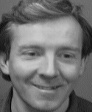
\includegraphics[scale=1]{Blur_original}
    
\includegraphics[scale=1]{Blur}
    \caption{Imagen antes y después de un proceso de \textit{blurring}}
    \label{im:Blur}
\end{figure}

\subsection{Comparación de redes neuronales}
EL resultado de nuestra prueba se compara con el trabajo de \cite{mcpherson2016defeating} donde se muestra resultados en TOP 1 donde solo se evalúa al primer resultado mas cercano. La única base de datos que usa es AT\&T descrita en la sección \ref{Att}.

Para replicar su experimento usamos la misma cantidad de datos de entrenamiento (8 imágenes por sujeto) y prueba (2 imágenes por sujeto). 
Todos los rostros fueron ofuscados antes de las pruebas, usado un Kernel Gaussiano de tamaño 64 para asemejarse al ofuscamiento usado por McPherson. 

En este proceso de experimentación se localizan los punto fiduciales en la imagen de entrenamiento y se alinean en la imagen ofuscada, debido a que en la imagen ofuscada no es posible encontrar puntos con la propuesta. Luego de la alineación de puntos se extraen las caracterizaras siguiendo el curso normal del proceso de reconocimiento teniendo una mejora 26\% en el reconocimiento.

\begin{table}[]
\centering
\caption{Comparación entre propuesta y método propuesto en \cite{mcpherson2016defeating}}
\label{ta::Blurred}
\begin{tabular}{|l|c|}
\hline
\textbf{Metodo}    & \textbf{Blurred Top 1} \\ \hline
\textbf{McPherson} & 57.75\%                \\ \hline
\textbf{Propuesta} & 83.42\%                \\ \hline
\end{tabular}
\end{table}

Como se observa en el Cuadro \ref{ta::Blurred} la propuesta de esta tesis es superior al resultado obtenido por \cite{mcpherson2016defeating}, esto se puede explicar al hecho que el proceso de \textit{blurring} dispersa la información con el uso del kernel Gaussiano y las mascaras de Gabor las reúne para el proceso de reconocimiento. También la aplicación de \textit{blurring} sobre la imagen del rostro a procesar no parece afectar la recolección de información en el espacio de la señales obtenidas tras la aplicación de las mascaras de Gabor. Finalmente hay que destacar que a diferencia del resto de pruebas, en esta se tienen 8 imágenes de entrenamiento un numero mucho mayor que permite una mayor tasa de aciertos.
	
\section{Consideraciones Finales}

La propuesta ha logrado adaptar \ac{EBGM} a un contexto de vídeo vigilancia gracias al reemplazo del uso de modelos para detectar los puntos de donde extraer características con \ac{CLNF}, que es un detector basado en \ac{CLM} donde la detección de puntos se realiza con una red neuronal en cada punto y el resultado final es evaluado en conjunto para darle mayor robustez.

La adopción de nuestra propuesta mejora el porcentaje de 2\% de aciertos en las bases de datos Georgia y de 10\% y 6\% en las bases de datos obtenidas a partir de la cámara de seguridad.

Se ha realizado una evaluación de parámetros de \ac{EBGM} donde se ha detallado varias formas de influir en el resultados final de \ac{EBGM}.  

Finalmente se menciona todas las opciones experimentadas para producir el \textit{pipeline} final que presenta este trabajo de tesis.
